
\section{Artificial Neural Networks (ANN)}
An ANN is a data-structure to define arbitrarily complex mathematical functions

\subsection{Artificial Neurons}
\begin{itemize}
    \item Receives an \textcolor{blue}{input vector $[x_1,x_2, ...]$}
    \item Each neuron has its own \textcolor{blue}{input weights $[w_1, w_2, ...]$} and \textcolor{blue}{bias b} (=intercept)
    \item Neuron calculates the sum of the weighted input (dot product $\vec{x} \cdot \vec{w}$), adds a bias b, and passes it through a \textcolor{blue}{nonlinear activation function}
\end{itemize}
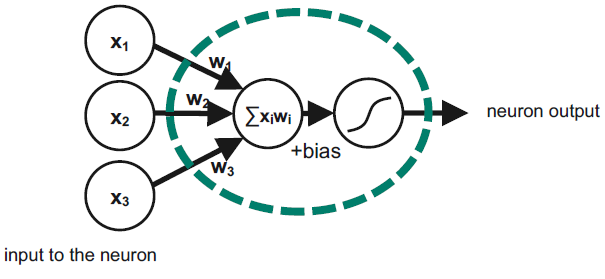
\includegraphics[width=0.6\linewidth]{artificial_neurons-1.png} \\

\textbf{Activation Function (ReLU)}

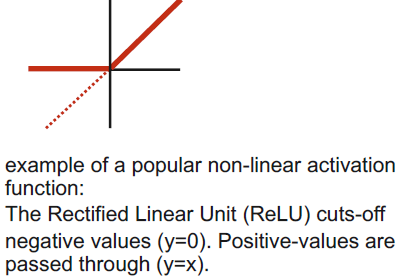
\includegraphics[width=0.6\linewidth]{artificial_neurons-2.png}


\subsection{Simple Artificial Neural Network (ANN)}
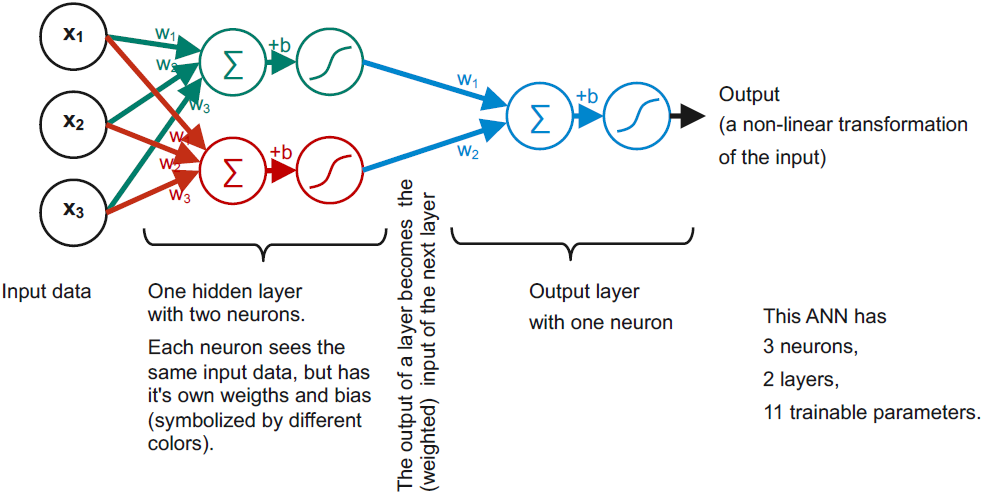
\includegraphics[width=\linewidth]{ann.png}

\textcolor{blue}{Trainable parameters} input vectors and input weights

\subsection{Training an ANN}
\textbf{Supervised learning}
\begin{itemize}
    \item Data with label
    \item For each input $\vec{x}$ we are given the output $\vec{y}$
    \item ANN is initialized with random weights
    \item An optimizer (e.g. SGD) reduces a cost-function (e.g. MSE)
    \item \textcolor{blue}{At every iteration, and for every single weight $w$ and bias $b$, the partial derivative needs to be calculated.} (Backpropagation algorithm)
\end{itemize}
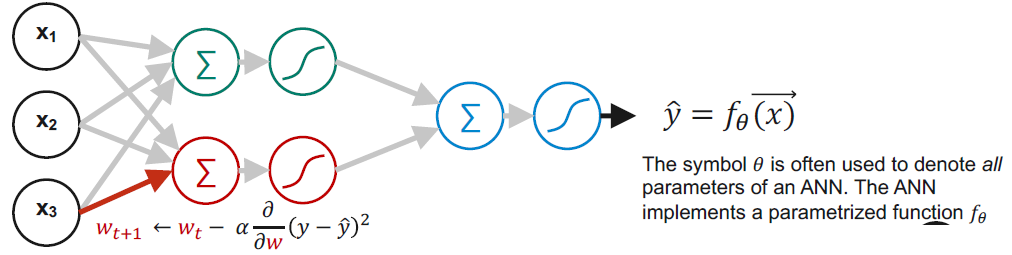
\includegraphics[width=\linewidth]{train_ann.png}
